\documentclass[11pt]{article}
\usepackage{amsfonts}
\usepackage{amssymb}
\usepackage{geometry}
\usepackage{graphicx}
\usepackage{wrapfig}
\usepackage{tikz}
\usetikzlibrary{arrows.meta}
\usepackage{amsmath}
\usepackage{xcolor}
\usepackage[utf8]{inputenc}
\usepackage[T1]{fontenc}
\usepackage{caption}
\usepackage{fancyhdr}
\usepackage{fontawesome5}
\usepackage[inline]{enumitem}
\usepackage{array}
\usepackage[table]{xcolor}
\usepackage{colortbl}
\usepackage{mdframed}
\usepackage[most]{tcolorbox}
\usepackage{soul}
\graphicspath{{task/}}
\definecolor{ncertblue}{RGB}{204, 232, 247}
\setlength{\headheight}{20pt}
\sloppy



\geometry{a4paper, margin=1in}

\fancypagestyle{firstpage}{
    \fancyhf{}
    \fancyhead[L]{\includegraphics[height=1.4cm]{../../iiitb_logo.png}}
    \fancyhead[R]{%
        \begin{tabular}{r}
            \textbf{Name:} Pirjade Sabahat Rehan\\
            \textbf{ID:} COMETFWC056\\
            \textbf{Date:} January 26, 2026
        \end{tabular}
    }
    \renewcommand{\headrulewidth}{0.6pt}
}
\pagestyle{plain}
\begin{document}
\thispagestyle{firstpage}
\vspace*{0.5cm}
\begin{center}
    \huge\textcolor{cyan}{\textbf{\huge RELATIONS AND FUNCTIONS}}
\end{center}
\begin{center}
\begin{tcolorbox}[
  enhanced,
  width=0.25\textwidth,   
  colback=cyan!20,
  colframe=cyan!80!black,
  boxrule=1.2pt,
  arc=0mm,                
  left=10pt,
  right=10pt,
  top=8pt,
  bottom=8pt
]
\centering
\textbf{\textcolor{cyan!80!black}{EXERCISE 2.1}}
\end{tcolorbox}
\end{center}
\begin{enumerate}[label=\arabic*., leftmargin=0pt, itemsep=0.6em]

\item If $\left(\frac{x}{3}+1, y-\frac{2}{3}\right)=\left(\frac{5}{3}, \frac{1}{3}\right)$,
find the values of $x$ and $y$.

\item If the set $A$ has 3 elements and the set $B=\{3,4,5\}$, find the number of
elements in $(A\times B)$.

\item If $G=\{7,8\}$ and $H=\{5,4,2\}$, find $G\times H$ and $H\times G$.

\item State whether each of the following statements are true or false.
If false, rewrite the statement correctly.
\begin{enumerate}[label=(\roman*), leftmargin=1.2em]
\item If $P=\{m,n\}$ and $Q=\{n,m\}$, then $P\times Q=\{(m,n),(n,m)\}$.
\item If $A$ and $B$ are non-empty sets, then $A\times B$ is a non-empty set
of ordered pairs $(x,y)$ such that $x\in A$ and $y\in B$.
\item If $A=\{1,2\}$, $B=\{3,4\}$, then $A\times(B\cap\phi)=\phi$.
\end{enumerate}

\item If $A=\{-1,1\}$, find $A\times A\times A$.

\item If $A\times B=\{(a,x),(a,y),(b,x),(b,y)\}$, find $A$ and $B$.

\item Let $A=\{1,2\}$, $B=\{1,2,3,4\}$, $C=\{5,6\}$ and $D=\{5,6,7,8\}$.
Verify that:
\begin{enumerate}[label=(\roman*), leftmargin=1.2em]
\item $A\times(B\cap C)=(A\times B)\cap(A\times C)$
\item $A\times C$ is a subset of $B\times D$.
\end{enumerate}

\item Let $A=\{1,2\}$ and $B=\{3,4\}$. Write $A\times B$.
How many subsets does $A\times B$ have? List them.

\item Let $A$ and $B$ be sets such that $n(A)=3$ and $n(B)=2$.
If $(x,1),(y,2),(z,1)\in A\times B$, find $A$ and $B$.

\item The Cartesian product $A\times A$ has 9 elements including
$(-1,0)$ and $(0,1)$. Find the set $A$ and the remaining elements of $A\times A$.

\end{enumerate}

\textcolor{cyan}{\section*{2.3 Relations}}

\begin{wrapfigure}[8]{r}{0.40\textwidth}
\centering
\vspace{-25pt} 
\begin{tikzpicture}[>=Stealth, scale=0.7]

\draw[very thick, fill=ncertblue] (-2.5,0) ellipse (1.0 and 2.5);
\node at (-2.5,2.8) {\textbf{P}};
\node (a) at (-2.5,1.2) {$\bullet\ a$};
\node (b) at (-2.5,0.2) {$\bullet\ b$};
\node (c) at (-2.5,-0.8) {$\bullet\ c$};

\draw[very thick, fill=ncertblue] (2.5,0) ellipse (1.5 and 3.0);
\node at (2.5,3.3) {\textbf{Q}};
\node (ali) at (2.5,1.5) {$\bullet$ Ali};
\node (bha) at (2.5,0.7) {$\bullet$ Bhanu};
\node (bin) at (2.5,-0.1) {$\bullet$ Binoy};
\node (cha) at (2.5,-0.9) {$\bullet$ Chandra};
\node (div) at (2.5,-1.7) {$\bullet$ Divya};

\draw[->, thick] (-1.7,1.2) -- (1.2,1.5);
\draw[->, thick] (-1.7,0.2) -- (1.2,0.7);
\draw[->, thick] (-1.7,0.2) -- (1.2,-0.1);
\draw[->, thick] (-1.7,-0.8) -- (1.2,-0.9);
\end{tikzpicture}
\caption*{\textbf{Fig 2.4}}
\end{wrapfigure}

Consider the two sets $P = \{a, b, c\}$ and $Q = \{\text{Ali, Bhanu, Binoy, Chandra, Divya}\}$. The Cartesian product of $P$ and $Q$ has 15 ordered pairs: $P \times Q = \{(a, \text{Ali}), (a, \text{Bhanu}), \dots, (c, \text{Divya})\}$. 


We can now obtain a subset of $P \times Q$ by introducing a relation $R$ as:
$R = \{ (x,y) : x \text{ is the first letter of the name } y, x \in P, y \in Q \}$. 


Then $R = \{(a, \text{Ali}), (b, \text{Bhanu}), (b, \text{Binoy}), (c, \text{Chandra})\}$.
An arrow diagram of this relation $R$ is shown in Fig.~2.4.\\
{\setlength{\parindent}{0pt}
\colorbox{ncertblue}{\textcolor{cyan}{\textbf{Definition 2}}}\hspace{0.5em}
A relation $R$ from a non-empty set $A$ to a non-empty set $B$ is a subset of the
cartesian product $A \times B$. The subset is derived by describing a
relationship between the first element and the second element of the ordered
pairs in $A \times B$. The second element is called the \textit{image} of the
first element.
}

\vspace{0.6em}
\noindent
\colorbox{ncertblue}{\textcolor{cyan}{\textbf{Definition 3}}}\hspace{0.5em}
The set of all first elements of the ordered pairs in a relation $R$ from a set
$A$ to a set $B$ is called the \textit{domain} of the relation $R$.

\vspace{0.6em}
\noindent
\colorbox{ncertblue}{\textcolor{cyan}{\textbf{Definition 4}}}\hspace{0.5em}
The set of all second elements in a relation $R$ from a set $A$ to a set $B$ is
called the \textit{range} of the relation $R$. The whole set $B$ is called the
\textit{codomain} of the relation $R$. Note that range $\subset$ codomain.

\vspace{0.6em}
\noindent
\colorbox{ncertblue}{\textcolor{cyan}{\textbf{\textit{Remarks}}}}

\begin{enumerate}
\item A relation may be represented algebraically either by the
\textit{Roster method} or by the \textit{Set-builder method}.
\item An arrow diagram is a visual representation of a relation.
\end{enumerate}

\noindent\textcolor{cyan}{\textbf{Example 7}}

\textbf{Let $A=\{1,2,3,4,5,6\}$.} Define a relation $R$ from $A$ to $A$ by 
$R=\{(x,y):y=x+1\}$
\begin{enumerate}
    \item[(i)] Depict this relation using an arrow diagram.
    \item[(ii)] Write down the domain, codomain and range of $R$.
\end{enumerate}
\noindent\textcolor{cyan}{\textbf{Solution}}

\begin{minipage}[t]{0.58\textwidth}
\begin{enumerate}[label=(\roman*), leftmargin=1.5em, nosep]
\item By the definition of the relation,\\
$R=\{(1,2),(2,3),(3,4),(4,5),(5,6)\}$.\\
The corresponding arrow diagram is shown in Fig.~2.5.

\item We can see that the
domain $=\{1,2,3,4,5\}$,\\
the range $=\{2,3,4,5,6\}$,\\
and the codomain $=\{1,2,3,4,5,6\}$.
\end{enumerate}

\end{minipage}
\hfill
\begin{minipage}[t]{0.38\textwidth}
\vspace{0pt} 
\centering
\includegraphics[width=\linewidth]{2.5.jpg}
\end{minipage}
\vspace{0.6cm}
\textcolor{cyan}{\textbf{Example 8}}
 The Fig 2.6 shows a relation between the sets $P$ and $Q$. Write this relation 
\begin{enumerate}
    \item[(i)] in set-builder form, 
    \item[(ii)] in roster form. 
\end{enumerate}
What is its domain and range?\\


\textcolor{cyan}{\textbf{Solution}}  
It is obvious that the relation $R$ is “$x$ is the square of $y$”.

\par 

\noindent
\begin{minipage}[t]{0.58\textwidth}

\begin{enumerate}
\item[(i)] \textbf{In set-builder form,}
$R = \{(x,y) : x \text{ is the square of } y,\ x \in P,\ y \in Q\}$

\item[(ii)] \textbf{In roster form,}
$R = \{(9,3),(9,-3),(4,2),(4,-2),(25,5),(25,-5)\}$
\end{enumerate}

The domain of this relation is $\{4,9,25\}$.\\
The range of this relation is $\{-2,2,-3,3,-5,5\}$.\\
Note that the element $1$ is not related to any element in set $P$.
The set $Q$ is the codomain of this relation.

\end{minipage}
\hfill
\begin{minipage}[t]{0.38\textwidth}
\vspace{0pt} 
\centering
\includegraphics[width=\linewidth]{2.6.jpg}

\end{minipage}
\begin{tcolorbox}[
  enhanced,
  breakable,
  width=\textwidth,       
  colback=cyan!15,
  colframe=cyan!70!black,
  boxrule=1.2pt,           
  arc=2mm,
  left=16pt,              
  right=16pt,
  top=12pt,
  bottom=12pt,
  before skip=10pt,
  after skip=12pt
]

\textbf{\textcolor{cyan!70!black}{\faHandPointRight\ Note}}\quad
The total number of relations that can be defined from a set $A$ to a set $B$
is the number of possible subsets of $A \times B$. If $n(A)=p$ and $n(B)=q$, then

$n(A \times B)=pq$
and the total number of relations is $2^{pq}$.

\end{tcolorbox}


\vspace{0.75cm}
\noindent\textcolor{cyan}{\textbf{Example 9}}
Let $A = \{1, 2\}$ and $B = \{3, 4\}$. Find the number of relations from $A$ to $B$.

\noindent\textcolor{cyan}{\textbf{Solution}} We have,
$
A \times B = \{(1, 3), (1, 4), (2, 3), (2, 4)\}.
$
\noindent Since $n(A \times B) = 4$, the number of subsets of $A \times B$ is $2^4$. Therefore, the number of relations from $A$ into $B$ will be $2^4$.

\noindent
\begin{minipage}[t]{\linewidth}
\colorbox{ncertblue}{\textcolor{cyan}{\textbf{\textit{Remarks}}}}
 A relation $R$ from $A$ to $A$ is also stated as a relation on $A$.
\end{minipage}
\begin{center}
\begin{tcolorbox}[
  enhanced,
  width=0.25\textwidth,   
  colback=cyan!20,
  colframe=cyan!80!black,
  boxrule=1.2pt,
  arc=0mm,                
  left=10pt,
  right=10pt,
  top=8pt,
  bottom=8pt
]
\centering
\textbf{\textcolor{cyan!80!black}{EXERCISE 2.2}}
\end{tcolorbox}
\end{center}

\begin{enumerate}
    \item Let $A = \{1, 2, 3, \dots, 14\}$. Define a relation $R$ from $A$ to $A$ by $R = \{(x, y) : 3x - y = 0, \text{ where } x, y \in A\}$. Write down its domain, codomain and range.

    \item Define a relation $R$ on the set $\mathbb{N}$ of natural numbers by $R = \{(x, y) : y = x + 5, x \text{ is a natural number less than } 4; x, y \in \mathbb{N}\}$. Depict this relationship using roster form. Write down the domain and the range.

    \item $A = \{1, 2, 3, 5\}$ and $B = \{4, 6, 9\}$. Define a relation $R$ from $A$ to $B$ by $R = \{(x, y) : \text{the difference between } x \text{ and } y \text{ is odd}; x \in A, y \in B\}$. Write $R$ in roster form.

    \vspace{10pt}
    \begin{minipage}[t]{0.6\textwidth}
        \item The Fig 2.7 shows a relationship between the sets $P$ and $Q$. Write this relation
        \begin{enumerate}
            \item[(i)] in set-builder form
            \item[(ii)] in roster form.
        \end{enumerate}
        What is its domain and range?

        \vspace{10pt}
        \item Let $A = \{1, 2, 3, 4, 6\}$. Let $R$ be the relation on $A$ defined by 
        $\{(a, b) : a, b \in A, b \text{ is exactly divisible by } a\}$.
        \begin{enumerate}
            \item[(i)] Write $R$ in roster form
            \item[(ii)] Find the domain of $R$
            \item[(iii)] Find the range of $R$.
        \end{enumerate}
    \end{minipage}
    \hfill
    \begin{minipage}[t]{0.45\textwidth}
        \vspace{10pt}
        \centering
        \includegraphics[width=\textwidth]{2.7.jpg}

    \end{minipage}
    \vspace{10pt}
    \item Determine the domain and range of the relation $R$ defined by $R = \{(x, x + 5) : x \in \{0, 1, 2, 3, 4, 5\}\}$.

    \item Write the relation $R = \{(x, x^3) : x \text{ is a prime number less than } 10\}$ in roster form.

    \item Let $A = \{x, y, z\}$ and $B = \{1, 2\}$. Find the number of relations from $A$ to $B$.

    \item Let $R$ be the relation on $\mathbb{Z}$ defined by $R = \{(a, b) : a, b \in \mathbb{Z}, a - b \text{ is an integer}\}$. Find the domain and range of $R$.
\end{enumerate}

\noindent
\colorbox{ncertblue}{\textcolor{cyan}{\textbf{2.4}}}\hspace{6pt}
\textcolor{cyan}{\textbf{Functions}}
In this chapter, we studied relations and functions. It is one of the most important concepts in mathematics. We can visualise a function as a rule, which produces new elements out of some given elements. There are many terms such as ‘map’ or ‘mapping’ used to denote a function.

\vspace{10pt}
\noindent\colorbox{ncertblue}{\textcolor{cyan}{\textbf{Definition 5}}}\hspace{0.5em}
\noindent A relation $f$ from a set $A$ to a set $B$ is said to be a function if every element of set $A$ has one and only one image in set $B$.
\vspace{5pt}
 In other words, a function $f$ is a relation from a non-empty set $A$ to a non-empty set $B$ such that the domain of $f$ is $A$ and no two distinct ordered pairs in $f$ have the same first element.
\vspace{5pt}

If $f$ is a function from $A$ to $B$ and $(a, b) \in f$, then $f(a) = b$, where $b$ is called the \textbf{image} of $a$ under $f$ and $a$ is called the \textbf{preimage} of $b$ under $f$.

 The function $f$ from $A$ to $B$ is denoted by $f: A \to B$.
\vspace{10pt}

 Looking at the previous examples, we can easily see that the relation in Example 7 is not a function because the element 6 has no image.

\vspace{5pt}
 Again, the relation in Example 8 is not a function because the elements in the domain are connected to more than one images. Similarly, the relation in Example 9 is also not a function. (Why?) In the examples given below, we will see many more relations some of which are functions and others are not.\\

 
\noindent \textcolor{cyan}{\textbf{Example 9}} Let $\mathbb{N}$ be the set of natural numbers and the relation $R$ be defined on $\mathbb{N}$ such that $R = \{(x, y) : y = 2x, x, y \in \mathbb{N}\}$.\\
What is the domain, codomain and range of $R$? Is this relation a function?\\



\noindent\textcolor{cyan}{\textbf{Example 10}} The domain of $R$ is the set of natural numbers $\mathbb{N}$. The codomain is also $\mathbb{N}$. The range is the set of even natural numbers.
Since every natural number $n$ has one and only one image, this relation is a function.\\

\noindent\textcolor{cyan}{\textbf{Example 11}}  
Consider the following relations. For each relation, determine whether it is a function or not, giving reasons.
\par
\begin{center}
(i)\quad $R = \{(2,1),(3,1),(4,2)\}$, (ii)\quad $R = \{(2,2),(2,4),(3,3),(4,4)\}$
\end{center}
\begin{center}
    (iii)\quad $R = \{(1,2),(2,3),(3,4),(4,5),(5,6),(6,7)\}$
\end{center}
\vspace{0.35cm}
\noindent\textcolor{cyan}{\textbf{Solution}}
\begin{enumerate*}[label=(\roman*), itemjoin=\quad, itemjoin*=\quad]
\item Since 2, 3, 4 are the elements of domain of $R$ having their unique images, this relation $R$ is a function.\\
\item Since the same first element 2 corresponds to two different images 2 and 4, this relation is not a function.\\
\item Since every element has one and only one image, this relation is a function.\\
\end{enumerate*}
\vspace{0.45cm}
\colorbox{ncertblue}{\textcolor{cyan}{\textbf{Definition 6}}} A function which has either $\mathbb{R}$ or one of its subsets as its range is called a real valued function. Further, if its domain is also either $\mathbb{R}$ or a subset of $\mathbb{R}$, it is called a real function.\\
 \textcolor{cyan}{\textbf{Example 12}} 
Let $\mathbb{N}$ be the set of natural numbers. Define a real valued function
$f : \mathbb{N} \to \mathbb{N}$ by $f(x) = 2x + 1$. Using this definition,
complete the table given below.

\begin{center}
    \renewcommand{\arraystretch}{1.4}
\begin{tabular}{|c|c|c|c|c|c|c|c|}
\hline
\rowcolor{ncertblue}
$x$ & 1 & 2 & 3 & 4 & 5 & 6 & 7 \\ \hline
\rowcolor{ncertblue}
$y$ & $f(1)=$ & $f(2)=$ & $f(3)=$ & $f(4)=$ & $f(5)=$ & $f(6)=$ & $f(7)=$ \\ \hline
\end{tabular}
\end{center}
\vspace{15pt}
\noindent \textcolor{cyan}{\textbf{Solution}} The completed table is given by:

\begin{center}
    \renewcommand{\arraystretch}{1.4}
\begin{tabular}{|c|c|c|c|c|c|c|c|}
\hline
\rowcolor{ncertblue}
$x$ & 1 & 2 & 3 & 4 & 5 & 6 & 7 \\ \hline
\rowcolor{ncertblue}
$y$ & $f(1)=3$ & $f(2)=5$ & $f(3)=7$ & $f(4)=9$ & $f(5)=11$ & $f(6)=13$ & $f(7)=15$ \\ \hline
\end{tabular}
\end{center}
\textcolor{cyan}{\subsection*{2.4.1 Some functions and their graphs}}

\noindent\textbf{(i) Identity function}  
Let $\mathbb{R}$ be the set of real numbers. Define the real valued function  
$f : \mathbb{R} \to \mathbb{R}$ by
$
y = f(x) = x \quad \text{for each } x \in \mathbb{R}.
$
Such a function is called the \emph{identity function}. Here, the domain and
range of $f$ are $\mathbb{R}$. The graph is a straight line as shown in Fig~2.8.
It passes through the origin.



\begin{center}
\includegraphics[width=0.45\textwidth]{2.8.jpg}
\end{center}

\noindent\textbf{(ii) Constant function}  
Define the function $f : \mathbb{R} \to \mathbb{R}$ by
$y = f(x) = c, \quad x \in \mathbb{R},$
where $c$ is a constant. Here, the domain of $f$ is $\mathbb{R}$ and its range
is $\{c\}$.

\begin{center}
\includegraphics[width=0.45\textwidth]{2.9.jpg}
\end{center}
The graph is a line parallel to the $x$-axis. For example, if $f(x) = 3$ for each
$x \in \mathbb{R}$, then its graph will be a line as shown in Fig.~2.9.


 
\noindent\textbf{(iii) Polynomial function}  
A function $f : \mathbb{R} \to \mathbb{R}$ is said to be a polynomial function if
for each $x \in \mathbb{R}$,
$y = f(x) = a_0 + a_1 x + a_2 x^2 + \cdots + a_n x^n,$
where $n$ is a non-negative integer and
$a_0, a_1, a_2, \ldots, a_n \in \mathbb{R}$.

The function defined by $f(x) = x^3 - x^2 + 2$ is a polynomial function,
whereas the functions defined by
$g(x) = x^4 + \dfrac{2}{x}$ and
$h(x) = \dfrac{x^{2/3}}{2} + 2x$
are not polynomial functions.

\noindent\textcolor{cyan}{\textbf{Example 13}}  
Define the function $f:\mathbb{R}\to\mathbb{R}$ by  
$y = f(x) = x^{2},\ x \in \mathbb{R}$.  
Complete the Table given below by using this definition.  
What is the domain and range of this function?  
Draw the graph of $f$.

\vspace{0.6em}


\begin{center}
\renewcommand{\arraystretch}{1.4}
\begin{tabular}{|c|c|c|c|c|c|c|c|c|c|}
\hline
\rowcolor{ncertblue}
$x$ & $-4$ & $-3$ & $-2$ & $-1$ & $0$ & $1$ & $2$ & $3$ & $4$ \\ \hline
\rowcolor{ncertblue}
$y=f(x)=x^{2}$ &  &  &  &  &  &  &  &  &  \\ \hline
\end{tabular}
\end{center}

\vspace{0.8em}


\noindent\textcolor{cyan}{\textbf{Solution}}  
The completed Table is given below:

\vspace{0.6em}
\begin{center}
\renewcommand{\arraystretch}{1.4}
\begin{tabular}{|c|c|c|c|c|c|c|c|c|c|}
\hline
\rowcolor{ncertblue}
$x$ & $-4$ & $-3$ & $-2$ & $-1$ & $0$ & $1$ & $2$ & $3$ & $4$ \\ \hline
\rowcolor{ncertblue}
$y=f(x)=x^{2}$ & 16 & 9 & 4 & 1 & 0 & 1 & 4 & 9 & 16 \\ \hline
\end{tabular}
\end{center}

\vspace{0.6em}

\noindent
Domain of $f = \{x : x \in \mathbb{R}\}$.  
Range of $f = \{x^{2} : x \in \mathbb{R}\}$.  
The graph of $f$ is given by Fig~2.10.

\vspace{0.8em}

\begin{center}
\includegraphics[width=0.45\textwidth]{2.10.jpg}

\textbf{Fig 2.10}
\end{center}

\vspace{0.5em}
\noindent\textcolor{cyan}{\textbf{Example 14}}  
Draw the graph of the function $f:\mathbb{R}\to\mathbb{R}$ defined by  
$f(x)=x^{3},\ x\in\mathbb{R}$.



\noindent\textcolor{cyan}{\textbf{Solution}}  
We have  
$f(0)=0,\ f(1)=1,\ f(-1)=-1,\ f(2)=8,\ f(-2)=-8,\ f(3)=27,\ f(-3)=-27$, etc.  
Therefore,
$
f=\{(x,x^{3}):x\in\mathbb{R}\}.
$
The graph of $f$ is given in Fig.~2.11.


\begin{center}
\includegraphics[width=0.45\textwidth]{2.11.jpg}
\end{center}

\noindent\textcolor{cyan}{\textbf{Example 15}}  
Define the real valued function
$
f : \mathbb{R}\setminus\{0\} \to \mathbb{R}
$
defined by $f(x)=\dfrac{1}{x},\ x\in\mathbb{R}\setminus\{0\}$, Complete the Table given below using this definition.
What is the domain and range of this function?



\begin{center}
\renewcommand{\arraystretch}{1.5}
\begin{tabular}{|c|c|c|c|c|c|c|c|c|c|}
\hline
\rowcolor{ncertblue}
$x$ & $-2$ & $-1.5$ & $-1$ & $-0.5$ & $0.25$ & $0.5$ & $1$ & $1.5$ & $2$ \\ \hline
\rowcolor{ncertblue}
$y=\dfrac{1}{x}$ & $\cdots$ & $\cdots$ & $\cdots$ & $\cdots$ & $\cdots$ & $\cdots$ & $\cdots$ & $\cdots$ & $\cdots$ \\ \hline
\end{tabular}
\end{center}



\noindent\textcolor{cyan}{\textbf{Solution}}  
The completed Table is given by


\begin{center}
\renewcommand{\arraystretch}{1.5}
\begin{tabular}{|c|c|c|c|c|c|c|c|c|c|}
\hline
\rowcolor{ncertblue}
$x$ & $-2$ & $-1.5$ & $-1$ & $-0.5$ & $0.25$ & $0.5$ & $1$ & $1.5$ & $2$ \\ \hline
\rowcolor{ncertblue}
$y=\dfrac{1}{x}$ &
$-0.5$ & $-0.67$ & $-1$ & $-2$ & $4$ & $2$ & $1$ & $0.67$ & $0.5$ \\ \hline
\end{tabular}
\end{center}



Domain of $f = \mathbb{R}\setminus\{0\}$.  
Range of $f = \mathbb{R}\setminus\{0\}$.
The domain of $f$ is all real numbers except $0$ and its range is also all real
numbers except $0$. The graph of $f$ is given in Fig~2.12.



\begin{center}
    \includegraphics[width=0.58\textwidth]{2.12.jpg}\\
\end{center}

\vspace{0.6cm}

\noindent
\begin{minipage}[t]{0.58\textwidth}

\noindent\textbf{(v) The Modulus function}

The function $f:\mathbb{R}\to\mathbb{R}$ defined by
$f(x)=|x|$ for each $x\in\mathbb{R}$ is called the
\emph{modulus function}. For each non-negative value of $x$,
$f(x)$ is equal to $x$. But for negative values of $x$, the value
of $f(x)$ is the negative of the value of $x$, i.e.,

$
f(x)=
\begin{cases}
x, & x\ge 0,\\
-x, & x<0.\\
\end{cases}
$

The graph of the modulus function is given in Fig.~2.13.

\end{minipage}
\hfill
\begin{minipage}[t]{0.38\textwidth}
\vspace{0pt} % CRITICAL for top alignment
\centering
\includegraphics[width=\linewidth]{2.13.jpg}

\end{minipage}

\vspace{0.6cm}



\vspace{0.6cm}
\noindent\textbf{(vi) Signum function}  
The function $f:\mathbb{R}\to\mathbb{R}$ defined by
$f(x)=\operatorname{sgn}(x)$ is called the \emph{signum function}.


\begin{align*}
f(x) &=
\begin{cases}
1, & x>0,\\
0, & x=0,\\
-1, & x<0.
\end{cases}
\end{align*}



The domain of the signum function is $\mathbb{R}$ and the range is
the set $\{-1,0,1\}$. The graph of the signum function is given by
Fig.~2.14.


\begin{center}
\includegraphics[width=0.55\textwidth]{2.14.jpg}
\end{center}


\noindent
\begin{minipage}[t]{0.58\textwidth}

\noindent\textbf{(vii) Greatest integer function}

The function $f:\mathbb{R}\to\mathbb{R}$ defined by  
$f(x)=[x],\ x\in\mathbb{R}$ assumes the value of the greatest integer,
less than or equal to $x$. Such a function is called the
\emph{greatest integer function}.



\begin{center}
$
\begin{aligned}
[x] &= -1, && -1 \le x < 0,\\
[x] &= \phantom{-}0, && 0 \le x < 1,\\
[x] &= \phantom{-}1, && 1 \le x < 2,\\
[x] &= \phantom{-}2, && 2 \le x < 3 \text{ and so on.}
\end{aligned}
$
\end{center}

The graph of the function is shown in Fig.~2.15.\\

\end{minipage}
\hfill
\begin{minipage}[t]{0.38\textwidth}
\vspace{0pt}
\centering
\includegraphics[width=\linewidth]{2.15.jpg}

\textbf{Fig 2.15}
\end{minipage}



\noindent
\textcolor{cyan}{\textbf{2.4.2 \quad Algebra of real functions}}\\


In this Section, we shall learn how to add two real functions, subtract a real
function from another, multiply a real function by a scalar (here by a scalar
we mean a real number), multiply two real functions and divide one real
function by another.


\noindent
\textbf{(i)\quad Addition of two real functions}  
Let $f : X \to \mathbb{R}$ and $g : X \to \mathbb{R}$ be any two real
functions, where $X \subset \mathbb{R}$. Then, we define
$(f+g) : X \to \mathbb{R}$ by

$(f+g)(x) = f(x) + g(x), \quad \text{for all } x \in X$.


\noindent
\textbf{(ii)\quad Subtraction of a real function from another}  
Let $f : X \to \mathbb{R}$ and $g : X \to \mathbb{R}$ be any two real
functions, where $X \subset \mathbb{R}$. Then, we define
$(f-g) : X \to \mathbb{R}$ by
\begin{align*}
(f-g)(x) &= f(x) - g(x), \quad \text{for all } x \in X.
\end{align*}


\noindent
\textbf{(iii)\quad Multiplication by a scalar}  
Let $f : X \to \mathbb{R}$ be a real valued function and $\alpha$ be a
scalar. Here by scalar, we mean a real number. Then the product
$\alpha f$ is a function from $X$ to $\mathbb{R}$ defined by
\begin{align*}
(\alpha f)(x) &= \alpha f(x), \quad x \in X.
\end{align*}


\noindent
\textbf{(iv)\quad Multiplication of two real functions}  
The product (or multiplication) of two real functions
$f : X \to \mathbb{R}$ and $g : X \to \mathbb{R}$ is a function
$fg : X \to \mathbb{R}$ defined by
\begin{align*}
(fg)(x) &= f(x)\,g(x), \quad \text{for all } x \in X.
\end{align*}

This is also called \emph{pointwise multiplication}.


\noindent
\textbf{(v)\quad Quotient of two real functions}  
Let $f$ and $g$ be two real functions defined from
$X \to \mathbb{R}$, where $X \subset \mathbb{R}$. The quotient of $f$ by
$g$ denoted by $\dfrac{f}{g}$ is a function defined by
\begin{align*}
\left(\frac{f}{g}\right)(x)
&= \frac{f(x)}{g(x)}, \quad
\text{provided } g(x) \neq 0,\ x \in X.
\end{align*}


\noindent\textcolor{cyan}{\textbf{Example 16}}  
Let $f(x) = x^{2}$ and $g(x) = 2x + 1$ be two real functions.
Find $(f+g)(x)$, $(f-g)(x)$, \\
$(fg)(x)$ and
$\left(\dfrac{f}{g}\right)(x)$.\\


\noindent\textcolor{cyan}{\textbf{Solution}}  
We have,\\

$
\begin{aligned}
(f+g)(x) &= x^{2} + 2x + 1,\\
(f-g)(x) &= x^{2} - 2x - 1,\\[0.5em]
(fg)(x) &= x^{2}(2x+1) = 2x^{3} + x^{2},\\
\left(\frac{f}{g}\right)(x) &= \frac{x^{2}}{2x+1},
\quad x \neq -\frac{1}{2}.
\end{aligned}
$



\noindent\textcolor{cyan}{\textbf{Example 17}}  
Let $f(x) = \sqrt{x}$ and $g(x) = x$ be two functions defined over the set
of non-negative real numbers. Find $(f+g)(x)$, $(f-g)(x)$, $(fg)(x)$ and
$\left(\dfrac{f}{g}\right)(x)$.



\noindent\textcolor{cyan}{\textbf{Solution}}  
We have,
\begin{align*}
(f+g)(x) &= \sqrt{x} + x,\\
(f-g)(x) &= \sqrt{x} - x,\\[0.5em]
(fg)(x) &= \sqrt{x}\,x = x^{3/2},\\
\left(\frac{f}{g}\right)(x) &= \frac{\sqrt{x}}{x} = x^{-1/2},
\quad x \neq 0.
\end{align*}

\newpage

\begin{center}
\begin{tcolorbox}[
  enhanced,
  width=0.25\textwidth,   
  colback=cyan!20,
  colframe=cyan!80!black,
  boxrule=1.2pt,
  arc=0mm,               
  left=10pt,
  right=10pt,
  top=8pt,
  bottom=8pt
]
\centering
\textbf{\textcolor{cyan!80!black}{EXERCISE 2.3}}
\end{tcolorbox}
\end{center}

\begin{enumerate}

\item Which of the following relations are functions? Give reasons.
If it is a function, determine its domain and range.\\
\begin{enumerate*}[label=(\roman*), itemjoin=\quad, itemjoin*=\quad]
\item $\{(2,1),(5,1),(8,1),(11,1),(14,1),(17,1)\}$\\
\item $\{(2,1),(4,2),(6,3),(8,4),(10,5),(12,6),(14,7)\}$\\
\item $\{(1,3),(1,5),(2,5)\}$
\end{enumerate*}


\item Find the domain and range of the following real functions:\\
\begin{enumerate*}[label=(\roman*), itemjoin=\quad, itemjoin*=\quad]
\item $f(x) = -|x|$
\item $f(x) = \sqrt{9 - x^{2}}$
\end{enumerate*}



\item A function $f$ is defined by $f(x) = 2x - 5$. Write down the values of\\
\begin{enumerate*}[label=(\roman*), itemjoin=\quad, itemjoin*=\quad]
\item $f(0)$
\item $f(7)$
\item $f(-3)$
\end{enumerate*}



\item The function $t$ which maps temperature in degree Celsius into temperature
in degree Fahrenheit is defined by
$
t(C) = \frac{9C}{5} + 32.
$
Find
\begin{enumerate*}[label=(\roman*), itemjoin=\quad, itemjoin*=\quad]
\item $t(0)$
\item $t(28)$
\item $t(-10)$
\item The value of $C$, when $t(C) = 212$
\end{enumerate*}


\item Find the range of each of the following functions:\\
\begin{enumerate*}[label=(\roman*), itemjoin=\quad, itemjoin*=\quad]\\
\item $f(x) = 2 - 3x,\ x \in \mathbb{R},\ x > 0$\\
\item $f(x) = x^{2} + 2$, $x$ is a real number\\
\item $f(x) = x$, $x$ is a real number
\end{enumerate*}

\end{enumerate}

\newpage
\begin{center}
    \huge\textcolor{cyan}{\huge\textbf{Miscellaneous Examples}}\\
\end{center}
\noindent\textcolor{cyan}{\textbf{Example 18}}\\

\noindent
\begin{wrapfigure}{r}{0.38\textwidth}
\vspace{-12pt} 
\centering
\includegraphics[width=\linewidth]{2.16.jpg}
\end{wrapfigure}
Let $\mathbb{R}$ be the set of real numbers.  
Define the real function
$f:\mathbb{R}\to\mathbb{R}, \quad f(x)=x+10$
and sketch the graph of this function.\\


\textcolor{cyan}{\textbf{Solution}}  
Here $f(0)=10$, $f(1)=11$, $f(2)=12$, $\ldots$,  
$f(10)=20$, etc., and  
$f(-1)=9$, $f(-2)=8$, $\ldots$, $f(-10)=0$ and so on.

\par
Therefore, the shape of the graph of the given function
assumes the form as shown in Fig.~2.16.\\

\textcolor{cyan}{\textbf{Remark}}  
The function $f$ defined by $f(x)=mx+c$, $x\in\mathbb{R}$,
is called a \emph{linear function}, where $m$ and $c$ are
constants. Above function is an example of a linear
function.\\

\noindent\textcolor{cyan}{\textbf{Example 19}}
Let $R$ be a relation from $\mathbb{Q}$ to $\mathbb{Q}$ defined by
$R=\{(a,b): a,b\in\mathbb{Q}\ \text{and } a-b\in\mathbb{Z}\}.$
Show that
\begin{enumerate}
\item $(a,a)\in R$ for all $a\in\mathbb{Q}$
\item $(a,b)\in R$ implies that $(b,a)\in R$
\item $(a,b)\in R$ and $(b,c)\in R$ implies that $(a,c)\in R$
\end{enumerate}

\noindent\textcolor{cyan}{\textbf{Solution}}
\begin{enumerate}
\item Since, $a-a=0\in\mathbb{Z}$, it follows that $(a,a)\in R$.
\item $(a,b)\in R$ implies that $a-b\in\mathbb{Z}$. So, $b-a\in\mathbb{Z}$.
Therefore, $(b,a)\in R$.
\item $(a,b)$ and $(b,c)\in R$ implies that $a-b\in\mathbb{Z}$.
$b-c\in\mathbb{Z}$. So,

\begin{center}
$(a-c)=(a-b)+(b-c)\in\mathbb{Z}.$
\end{center}

Therefore, $(a,c)\in R$.
\end{enumerate}


\noindent\textcolor{cyan}{\textbf{Example 20}}
Let $f=\{(1,1),(2,3),(0,-1),(-1,-3)\}$ be a linear function from
$\mathbb{Z}$ into $\mathbb{Z}$. Find $f(x)$.\\



\noindent\textcolor{cyan}{\textbf{Solution}}
Since $f$ is a linear function, $f(x)=mx+c$.
Also, since $(1,1),(0,-1)\in R$,
$f(1)=m+c=1 \quad \text{and} \quad f(0)=c=-1.$
This gives $m=2$ and $f(x)=2x-1$.\\

\par
\noindent\textcolor{cyan}{\textbf{Example 21}}
Find the domain of the function
$
\displaystyle
f(x)=\frac{x^{2}+3x+5}{x^{2}-5x+4}.$\\



\noindent\textcolor{cyan}{\textbf{Solution}}
Since $x^{2}-5x+4=(x-4)(x-1)$, the function $f$ is defined for all real
numbers except at $x=4$ and $x=1$.
Hence the domain of $f$ is
$
\mathbb{R}\setminus\{1,4\}.
$

\noindent\textcolor{cyan}{\textbf{Example 22}}  
The function $f$ is defined by
$
f(x)=
\begin{cases}
1-x, & x<0,\\[4pt]
1, & x=0,\\[4pt]
x+1, & x>0.
\end{cases}
$

Draw the graph of $f(x)$.

\par\begin{minipage}[t]{0.62\textwidth}
\vspace{0pt}
\textcolor{cyan}{\textbf{Solution}}  

Here, $f(x)=1-x$, $x<0$, this gives
\begin{center}
$
\begin{aligned}
f(-4) &= 1-(-4)=5;\\
f(-3) &= 1-(-3)=4;\\
f(-2) &= 1-(-2)=3;\\
f(-1) &= 1-(-1)=2; \text{ etc.,}
\end{aligned}
$
\end{center}


and
$f(1)=2,\quad f(2)=3,\quad f(3)=4,$
$f(4)=5 \text{and so on for} f(x)=x+1,\ x>0.$

Thus, the graph of $f$ is as shown in Fig.~2.17.
\end{minipage}
\hfill
\begin{minipage}[t]{0.4\textwidth}
\vspace{0pt}
\centering
\includegraphics[width=\linewidth]{2.17.jpg}

\end{minipage}


\vspace{0.8cm}
\newpage
\begin{center}
{\huge\color{cyan}\textit{Miscellaneous Exercise on Chapter 2}}
\end{center}

\vspace{0.5cm}

\begin{enumerate}

\item The relation $f$ is defined by
$
f(x)=
\begin{cases}
x^2, & 0 \le x \le 3,\\
3x, & 3 < x \le 10.
\end{cases}
$
The relation $g$ is defined by
$
g(x)=
\begin{cases}
x^2, & 0 \le x \le 2,\\
3x, & 2 \le x \le 10.
\end{cases}
$
Show that $f$ is a function and $g$ is not a function.

\item If $f(x)=x^2$, find
$
\dfrac{f(1.1)-f(1)}{1.1-1}.
$


\item Find the domain of the function
$
f(x)=\dfrac{x^2+2x+1}{x^2-8x+12}.
$

\item Find the domain and the range of the real function $f$ defined by
$
f(x)=\sqrt{x-1}.
$

\item Find the domain and the range of the real function $f$ defined by
$
f(x)=|x-1|.
$

\item Let
$
f=\left\{\left(x,\dfrac{x^2}{1+x^2}\right):x\in \mathbb{R}\right\}
$
be a function from $\mathbb{R}$ into $\mathbb{R}$. Determine the range of $f$.

\item Let $f,g:\mathbb{R}\to\mathbb{R}$ be defined, respectively, by
$f(x)=x+1,\quad g(x)=2x-3.$
Find $f+g$, $f-g$ and $\dfrac{f}{g}$.

\item Let
$
f=\{(1,1),(2,3),(0,-1),(-1,-3)\}
$
be a function from $\mathbb{Z}$ to $\mathbb{Z}$ defined by
$
f(x)=ax+b,
$
for some integers $a,b$. Determine $a$ and $b$.

\item Let $R$ be a relation from $\mathbb{N}$ to $\mathbb{N}$ defined by
$
R=\{(a,b):a,b\in\mathbb{N}\text{ and }a=b^2\}.
$
Are the following true?

\begin{enumerate}

\item $(a,a)\in R$, for all $a\in\mathbb{N}$
\item $(a,b)\in R$ implies $(b,a)\in R$
\item $(a,b)\in R$, $(b,c)\in R$ implies $(a,c)\in R$
\end{enumerate}
Justify your answer in each case.

\item Let $A=\{1,2,3,4\}$, $B=\{1,5,9,11,15,16\}$ and
$
f=\{(1,5),(2,9),(3,1),(4,5),(2,11)\}.
$
Are the following true?
\begin{enumerate}
\item $f$ is a relation from $A$ to $B$
\item $f$ is a function from $A$ to $B$
\end{enumerate}
Justify your answer in each case.

\item Let $f$ be the subset of $\mathbb{Z}\times\mathbb{Z}$ defined by
$
f=\{(ab,a+b):a,b\in\mathbb{Z}\}.
$
Is $f$ a function from $\mathbb{Z}$ to $\mathbb{Z}$? Justify your answer.

\item Let $A=\{9,10,11,12,13\}$ and let $f:A\to\mathbb{N}$ be defined by
$
f(n)=\text{the highest prime factor of }n.
$
Find the range of $f$.

\end{enumerate}

\vspace{0.5cm}
\begin{mdframed}[
  backgroundcolor=cyan!15,
  linecolor=cyan!40,
  linewidth=0pt,
  leftmargin=0pt,
  rightmargin=0pt,
  innerleftmargin=14pt,
  innerrightmargin=14pt,
  innertopmargin=12pt,
  innerbottommargin=12pt,
  skipabove=10pt,
  skipbelow=10pt,
  split=true
]
\begin{center}
{\bfseries\textcolor{cyan!60!black}{Summary}}
\end{center}

In this Chapter, we studied about relations and functions.
The main features of this Chapter are as follows:

\begin{itemize}[label=$\diamond$]

\item \textbf{Ordered pair}  
A pair of elements grouped together in a particular order.

\item \textbf{Cartesian product}  
$A \times B$ of two sets $A$ and $B$ is given by  
$A \times B = \{(a,b): a \in A, b \in B\}$.

In particular  
$R \times R = \{(x,y): x,y \in R\}$  

and  
$R \times R \times R = \{(x,y,z): x,y,z \in R\}$.

\item If $(a,b) = (x,y)$, then $a = x$ and $b = y$.

\item If $n(A) = p$ and $n(B) = q$, then $n(A \times B) = pq$.

\item $A \times \phi = \phi$.

\item In general, $A \times B \neq B \times A$.

\item \textbf{Relation}  
A relation $R$ from a set $A$ to a set $B$ is a subset of the cartesian product
$A \times B$ obtained by describing a relationship between the first element
$x$ and the second element $y$ of the ordered pairs in $A \times B$.

\item The \textit{image} of an element $x$ under a relation $R$ is given by $y$,
where $(x,y) \in R$.

\item The \textit{domain} of $R$ is the set of all first elements of the ordered
pairs in a relation $R$.

\item The \textit{range} of the relation $R$ is the set of all second elements of
the ordered pairs in a relation $R$.

\item \textbf{Function}  
A function $f$ from a set $A$ to a set $B$ is a specific type of relation for which
every element $x$ of set $A$ has one and only one image $y$ in set $B$.  
We write $f : A \to B$, where $f(x) = y$.

\item $A$ is the domain and $B$ is the codomain of $f$.

\item The range of the function is the set of images.

\item A real function has the set of real numbers or one of its subsets both as
its domain and as its range.

\item \textbf{\textit{Algebra of functions}}  
For functions $f : X \to \mathbb{R}$ and $g : X \to \mathbb{R}$, we have

$
\begin{aligned}
(f+g)(x) &= f(x) + g(x), && x \in X,\\
(f-g)(x) &= f(x) - g(x), && x \in X,\\
(f\cdot g)(x) &= f(x)\cdot g(x), && x \in X,\\
(kf)(x) &= k(f(x)), && x \in X,\ \text{where } k \text{ is a real number},\\
\left(\frac{f}{g}\right)(x) &= \frac{f(x)}{g(x)}, && x \in X,\ g(x) \neq 0.
\end{aligned}
$


\end{itemize}

\end{mdframed}
\begin{mdframed}[
  backgroundcolor=cyan!15,
  linecolor=cyan!40,
  linewidth=0pt,
  leftmargin=0pt,
  rightmargin=0pt,
  innerleftmargin=14pt,
  innerrightmargin=14pt,
  innertopmargin=12pt,
  innerbottommargin=12pt,
  skipabove=10pt,
  skipbelow=10pt,
  split=true]

\begin{center}
\textcolor{cyan!60!black}{\textbf{\textit{Historical Note}}}
\end{center}

The word \textbf{FUNCTION} first appears in a Latin manuscript
\textit{``Methodus tangentium inversa, seu de functionibus''}
written by Gottfried Wilhelm Leibnitz (1646--1716) in 1673; Leibnitz
used the word in the non-analytical sense. He considered a function in
terms of ``mathematical job'' --- the ``employee'' being just a curve.



On July 5, 1698, Johan Bernoulli, in a letter to Leibnitz, for the first
time deliberately assigned a specialised use of the term
\textit{function} in the analytical sense. At the end of that month,
Leibnitz replied showing his approval.


\textit{Function} is found in English in 1779 in Chambers' Cyclopaedia:
``The term function is used in algebra, for an analytical expression any
way compounded of a variable quantity, and of numbers, or constant
quantities''.

\end{mdframed}

\begin{center}
\begin{tikzpicture}
  \draw[cyan!70!black, line width=0.6pt] (-2.8,0) -- (-0.9,0);

  \foreach \x/\y in {0/0.15,0/-0.15,0.15/0,-0.15/0} {
    \draw[cyan!70!black, fill=cyan!70!black]
      (\x,\y) -- ++(0.12,0.12) -- ++(-0.12,0.12)
      -- ++(-0.12,-0.12) -- cycle;
  }

  \draw[cyan!70!black, line width=0.6pt] (0.9,0) -- (2.8,0);
\end{tikzpicture}
\end{center}

\end{document}

